\section{Generality}
\label{sec:generality}

Although this paper examines the methodology as depicted in Figure~\ref{fig:workflow} on Kepler architecture and shows its performance optimizations for SGEMM, we argue that the developed toolchain can be easily extended to other NVIDIA GPUs and the explored optimization strategies is applicable to other floating-point computation-intensive applications.

{\em {\bf Generality of Toolchains}}: For a given new GPU architecture, users only need to regenerated disassembly codes with CUDA binary utilities, and then feed them to the solvers, which are portable among different GPU architecture. We have validated the functionalities of the solvers on Fermi, Kepler, Maxwell GPUs. The new assembler can be obtained by modifying the instruction grammar definition decoded by the solvers. In fact, this modification can be automatically generated with an assembler template~\cite{baldassin2005extending}.

{\em {\bf Generality of Optimizations}}: The optimization strategies include
FFMA dual-issue, register allocation, memory load/store width, and instruction
scheduling. The latter three strategies are applicable to other GPU
architectures by leveraging the benchmark to detect effective parameters. Only is
the first one specific to Kepler architecture. 

Note that the low-level optimizations are more microarchitectural specific than application specific. 
Usually, a float computation-intensive application can implemented using
blocking and tiling to improve computation memory access ratio and hide memory latency. As long as we use
register blocking, there will be multiple float computation instructions inside
the loop, then register allocation and dual issue can refer to SGEMM's
optimization in order to improve float computation throughput. 
%For instance,
The {\tt LDG.128} can reduce number of memory instructions, continous memory
access pattern applications can use this as well.
{\tt LDS.64} achieves best bandwidth on Kepler due to 8 bytes per shared memory bank. 
%We also vertified these two memory instruction achieve best for convolution algorithm.
The scheduling strategy is totally derived from instruction dependency and latency,
which is not specific to SGEMM. 
The instruction scheduling optimization requires support of assemble language.
In fact, the previous investigations of GEMM optimization on CPU have inspired
general performance tuning and compiler optimizations~\cite{lam1991cache}.  
%Although we use a exhaust search method to search the optimal scheduling, we
%argue that the idea may be applicable to general optimizations
%because small piece of code often occupy most of the
%execution time in a lot of scientific and engineering applications.
%As an alternative way, auto-tuning techniques~\cite{} 
%can be taken to find a better scheduling order. 
%For another floating-point intensive algorithm like convolution in deep learning applications, the FFMA throughput can be improved by eliminating register bank conflicts and activating dual issue. Then non-FFMA instructions are carefully scheduled without affecting the FFMA throughput. 

{\em {\bf Convolutional Algorithm Performance}}:
Our convolution algorithm implementation uses $128\times128$ shared memory blocking and
$8\times8$ register blocking. We optimize it at assembly-level using the method describe in section~\ref{sec:optimization}.
%The configuration of each layer can be found 
We benchmark three popular convolutional neural network:
Alexnet~\cite{krizhevsky2012imagenet}, Vgg~\cite{simonyan2014very} and
Overfeat~\cite{sermanet2013overfeat}.  The configuration of each convolutional
layer can be found in corresponding papers.
We compare the average convolution performance of all the convolutional layers in neural network. 
Figure~\ref{fig:conv} presents the performance of our optimized convolution. %The maximum convolution performance is 2653 Gflop/s.
Our convolution algorithm implementation is 39\%, 46\% and 62\% higher over cuDNN V4.0 for the three CNN configures on K20 GPU.

\begin{figure}[htbp]
\begin{center}
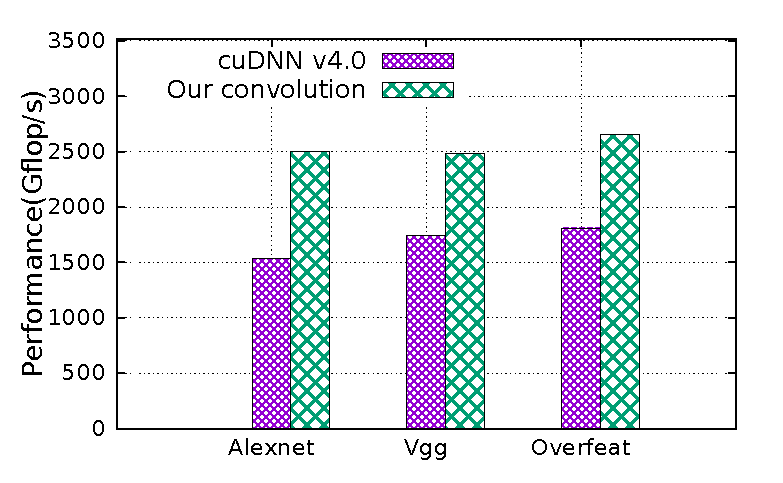
\includegraphics[scale=0.5]{cudnn}
    \caption{Performance comparison of cuDNN and our optimized convolution on K20 GPU(batch size is 128)}
\label{fig:conv}
\end{center}
\end{figure}
